\documentclass[a4paper,11pt]{article}
\usepackage[utf8]{inputenc}
\usepackage{listings}
\usepackage{amsmath}    % need for subequations
\usepackage{graphicx}   % need for figures
\usepackage{verbatim}   % useful for program listings
\usepackage{color}      % use if color is used in text
\usepackage{hyperref}  
\usepackage{url}
\usepackage{float}
\usepackage{todonotes}
\usepackage{tikz}
\usepackage{enumitem}
\usepackage{hyperref}
\usepackage{pdfpages}
\usepackage{caption}
\usepackage{subcaption}
\usepackage{listings}
\usepackage{color}
\usepackage{amsfonts}
\usepackage{latexsym}
\usepackage[T1]{fontenc} % use for allowing < and > in cleartext
\usepackage{fixltx2e}    % use for textsubscript

\usepackage[margin=2.5cm]{geometry}
\usepackage[ampersand]{easylist}
%\usepackage{epic,eepic}
\usepackage{tikz}

\bibliographystyle{plain}
\begin{document}
\setlength{\parindent}{0cm}
\setlength{\unitlength}{1mm}
\date{December 17th 2014\\ IT University of Copenhagen}
\title{Roles In Movies\\SAD2 Fall 2014}

\author{Sarah de Voss\\
\texttt{satv@itu.dk}
\and Elvis Flesborg\\
\texttt{efle@itu.dk}
\and Mads Westi\\
\texttt{mwek@itu.dk}}
\clearpage\maketitle
\newpage
\thispagestyle{empty}
\setcounter{page}{1}
\tableofcontents
\newpage

\section{Project Introduction}
So you want to make a movie? And you want it to be a movie with high ranking? We have the working hypothesis, that the success of the movie depends solely on what roles appear in the movie. With that in mind, we will look at the IMDB dataset, and find out what the correlation is between high ranking and the roles list of the movies.\\

Maybe it is one specific role that generates the high ranking, or it could be a pair, or triplet of the same roles, that do the trick.\\

In this project, we will try to find the correlation between a high ranking on IMDB and movie roles.\\

The solution to the problem should make room for creating a backend, that could answer these type of questions with some variables. Like: \\

\begin{easylist}[itemize]
& What 2 roles should be in my Horror movie, if it was the year 1983?
& What 3 roles should be in my Comedy, if it is the year 2014?
& What year should I have made an Animation movie with the two roles Policewoman, and Pedestrian?
\end{easylist} 

The code for our algorithm as well as this report is on Github on \url{https://github.com/MadsWesti/SAD2}. It is coded in Python3 and currently takes approximately 30 seconds to run on a normal laptop. \\

\subsection{Subproblems}
We have divided the problem into subproblems that we will look at as individual algorithmic problems. Their time complexities will also individually be looked at, and discussed.\\

\begin{easylist}[itemize]
& Make a data cleaning algorithm, that can link similarities (‘Police’, ‘Policewoman’, ‘Policeman’)
& Remove meta-characters like ‘Herself’, ‘Himself’, ‘Narrator’, etc…
& Put the role list through a thesaurus (for finding synonyms)
& What are the tendency curves for all years? (to see what roles are in, out, or steady.)
& What are the top role pairs instead of single roles?
\end{easylist}

\subsection{Algorithmic Solution}
We can create a simple solution, but it would probably not be very fast on a normal computer, so to optimize we make a streaming solution of the problem. Although one where the total length of the stream is known.\\

\subsection{Project Extension}
Due to limitations in memory, an extension to the streaming solution could be made. One that does not know the length of the stream beforehand.\\

We could find a more sophisticated algorithm in the course literature. This could help us get a better time complexity, but we must be sure about what we sacrifice in accuracy.\\

\subsection{Subproblems in the Project Extension}
\begin{easylist}[itemize]
& What are the top role triplets instead of pairs or singletons?
& Can we use the heavy hitters principle?
& Should we consider using MapReduce?
\end{easylist}


\section{Naïve solution to problem}
\subsection{Metrics for rankings}
The rankings in the IMDB database are within the interval 1 to 10. For every role, we will calculate a rank for that role in the following way:\\

Rank = $X \cdot \frac{n}{n+k} + C \cdot \frac{k}{n+k}$ \\ \\

where: \\
$X =$ average rating for the movie that the role appeared in\\
$n =$ number of movies that the role appeared in\\
$k =$ minimum number of movies required to be listed in the top 250\\
$C =$ the mean ranking across the entire database\\

This rank is the same weighted rank equation, that IMDB uses to rank their movies. \href{ftp://ftp.sunet.se/pub/tv+movies/imdb/ratings.list.gz}{IMDB ratings database} \\

\begin{easylist}[itemize]
& maybe a couple of lines about why this metric should be used, and if it’s a bad idea, and why:
& Compared to plain average
& Compared to maybe our own scale
\end{easylist}


\section{Simple solution to the stated problem}
At first we create a simple solution to the problem. One that does not have a complicated algorithm, but also runs through all the data. We then add the subproblems on top of this and analyze them individually.\\


\subsection{Adding subproblems}


\subsubsection{Data Cleaning Algorithm}
By looking at the data, and what roles are most frequently used, we have gathered information about some unwanted roles, and some cleaning, that we will have to do.\\

For every genre, there exists the roles ‘Himself’, ‘Herself’, ‘Narrator’, and ‘’. We are not interested in these, since they all represent a different entity, and if we come across one of these, we simply skip it.\\

Also, there are many roles that a present multiple times in the same move, and thus will have a rolename with a numbered suffix. eg. ‘Policeman \#1’. These role names will have to be counted as ‘Policeman’, and thus the suffix is stripped.\\

\begin{easylist}[itemize]
& String similarity: 
&& “Policewoman” vs “Policeman” 
&& “Nurse” vs. “Horse”
&& Make a weighted value for every 2 nearly similar words.
&&&  if abs(str1.length-str2.length) $<$  3, then run similarity\_check(str1, str2)
&&&  Maybe we can use the protein-alikeness algorithm from SAD1 course.
&&&  Maybe use Jaccard to match two words. 
\end{easylist}


\subsubsection{Synonyms}

\begin{easylist}[itemize]
& Check every role for synonyms.
& Find out how to check for ambiguity.
&& “Police” vs “Pigs”
&&& Could be same, but might not
&& “Policeman” vs “Policewoman”
&&& Does the gender matter in our algorithm, or do we not care.
& Maybe it makes the data worse, or less reliable
&& So should we include it?
& Link to an open thesaurus: \href{http://wordnet.princeton.edu/wordnet/download/current-version/}{princeton.edu}
\end{easylist}


\subsubsection{Tendency curves over the years}

\begin{easylist}[itemize]
& Make the role rank for every year
& Make definitions on when roles are on the rise, or the opposite, or steady every year.
&& Maybe we just have to look 5 years back, or maybe we should consider all years
& Consider exporting the data into a graphable format, for visualization
& Maybe cluster years together in decades? or 5-year clusters?
Role pairs
& Discuss how much the complexity rises
& Are there roles in the singleton solution that do not appear in these pairs?
&& roles that only work alone.
\end{easylist}

\subsubsection{Pairs in stead of Singletons}

\begin{easylist}[itemize]
& Take into account, doublegangers
&& Sort the tuples alphabetically, to avoid this
&& Find a reference to this in one of the slides.
& Show how much more space it fills
&& Show the aggregates for the different data structures
&&& \{movie1: [role1, role2, role3, role4], ranking\}
&&& \{role1: \{role2: [rank1, rank2, rank3]\}\}
&& Say how it sort of represents a graph.. draw the graph.
\end{easylist}

For any given simple undirected complete graph with $n$ vertices, there are $\frac{n(n-1)}{2} \Leftrightarrow \frac{n^2-n}{2}$ edges. If all the weights on the edges are equivalent to a set of the movies that link them, the space complexity will be $O (n^2 \cdot m)$. Where $m$ is the number of movies. \\

We create a toy example with 3 movies $(m_1, m_2, m_3)$, and 6 roles $(r_1, r_2, r_3, r_4, r_5, r_6)$. The overlap can be seen in figure \ref{fig:venn}. We save the data in two different structures in our algorithm. The first one is a dictionary, which contains the movies as indices and a list of roles as the value, see figure \ref{fig:aggregate_movies} for an aggregate. The data is thereafter converted into another dictionary, which are more like a graph type structure, see figure \ref{fig:aggregate_roles}. \\

The space complexity for the first aggregate is $O (m \cdot r)$, and the space complexity for the second aggregate is $ \sim (\frac{n^2-2}{2} \cdot m) \Rightarrow O (n^2 m)$.


\begin{figure}
\begin{center}
\begin{tikzpicture}
    \def\circleone{(90:1.75) circle (2.5)};
    \def\circletwo{(210:1.75) circle (2.5)};
    \def\circlethree{(330:1.75) circle (2.5)};
    \draw node {$r_1\ \ r_3$};
    \draw \circleone node[above] {$r_2$};
    \draw \circletwo node[below left] {$r_6$};
    \draw \circlethree node[below right] {$r_5$};
    \draw (270:1.75) node {$r_4$};
    \draw (90:4.5) node {$m_1$};
    \draw (210:4.7) node {$m_2$};
    \draw (330:4.7) node {$m_3$};
    \draw \circletwo;
    \draw \circlethree;
    \draw (-5,-5) rectangle (5,5);
\end{tikzpicture}
\caption{A venn diagram of the toy data}
\label{fig:venn}
\end{center}
\end{figure}

\begin{figure}
\begin{center}
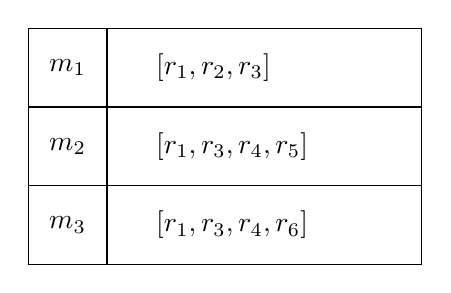
\begin{tikzpicture}
    \draw rectangle (1,1);
    \draw rectangle (1,2);
    \draw rectangle (1,3);
    \draw rectangle (5,1);
    \draw rectangle (5,2);
    \draw rectangle (5,3);

    \draw (.5,2.5) node {$m_1$};
    \draw (.5,1.5) node {$m_2$};
    \draw (.5,.5) node {$m_3$};

    \draw (1.5,2.5) node [right] {$[r_1, r_2, r_3]$};
    \draw (1.5,1.5) node [right] {$[r_1, r_3, r_4, r_5]$};
    \draw (1.5,.5) node [right] {$[r_1, r_3, r_4, r_6]$};
\end{tikzpicture}
\caption{Aggregate for the first data structure}
\label{fig:aggregate_movies}
\end{center}
\end{figure}

\begin{figure}
\begin{center}
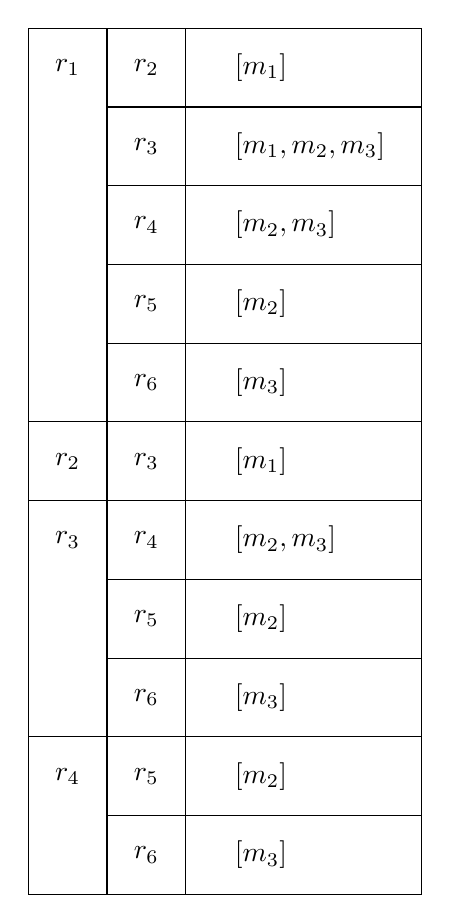
\begin{tikzpicture}
    \draw rectangle (5,11);

    \draw (0,0) rectangle (1,2);
    \draw (1,2) rectangle (1,5);
    \draw (1,5) rectangle (1,6);
    \draw (1, 6) rectangle (1,11);

    \draw rectangle (5,2);
    \draw rectangle (5,5);
    \draw rectangle (5,6);
    \draw rectangle (5,11);

    \foreach \x in {0,...,10} \draw (1,\x) rectangle (2,\x+1);
    \foreach \x in {0,...,10} \draw (2,\x) rectangle (5,\x+1);

    \draw (.5,10.5) node {$r_1$};
    \draw (.5,5.5) node {$r_2$};
    \draw (.5,4.5) node {$r_3$};
    \draw (.5,1.5) node {$r_4$};
    
    \draw (1.5,10.5) node {$r_2$};
    \draw (1.5,9.5) node {$r_3$};
    \draw (1.5,8.5) node {$r_4$};
    \draw (1.5,7.5) node {$r_5$};
    \draw (1.5,6.5) node {$r_6$};
    \draw (1.5,5.5) node {$r_3$};
    \draw (1.5,4.5) node {$r_4$};
    \draw (1.5,3.5) node {$r_5$};
    \draw (1.5,2.5) node {$r_6$};
    \draw (1.5,1.5) node {$r_5$};
    \draw (1.5,0.5) node {$r_6$};

    \draw (2.5,10.5) node [right] {$[m_1]$};
    \draw (2.5,9.5) node [right] {$[m_1, m_2, m_3]$};
    \draw (2.5,8.5) node [right] {$[m_2, m_3]$};
    \draw (2.5,7.5) node [right] {$[m_2]$};
    \draw (2.5,6.5) node [right] {$[m_3]$};
    \draw (2.5,5.5) node [right] {$[m_1]$};
    \draw (2.5,4.5) node [right] {$[m_2, m_3]$};
    \draw (2.5,3.5) node [right] {$[m_2]$};
    \draw (2.5,2.5) node [right] {$[m_3]$};
    \draw (2.5,1.5) node [right] {$[m_2]$};
    \draw (2.5,0.5) node [right] {$[m_3]$};
\end{tikzpicture}
\caption{Aggregate for the second data structure.}
\label{fig:aggregate_roles}
\end{center}
\end{figure}

\subsection{Space/time analysis}

\begin{easylist}[itemize]
& State complexity for all the subproblems
&& so all subproblems should be easily distinguishable in the code eg. have their own methods.
& Which subproblem algorithm has the largest space/time complexity
&& Where should we set in, to make it faster?
& Do we already sacrifice accuracy somewhere?
\end{easylist}


\section{Extended solution to problem}

\begin{easylist}[itemize]
& Choose a streaming solution with unknown stream length 
& Consider MapReduce - discuss why, and how.
\end{easylist}


\section{Discussion}


\section{Conclusion}
\end{document}
